\documentclass[letterpaper,twocolumn]{article}

\usepackage{listings}
\usepackage{pdflscape}
\usepackage{booktabs}
\usepackage{minted}
\newcommand\tab[1][1cm]{\hspace*{#1}}
\usepackage{graphicx} % Required for inserting images

\newcommand{\myparagraph}[1]{\vspace{0.1cm}\noindent \textbf{\textit{#1.}}}

\title{Project Title}
\date{}

\begin{document}


% TITLE PAGE
\begin{titlepage}
\newcommand{\HRule}{\rule{\linewidth}{0.5mm}} % Defines a new command for the horizontal lines, change thickness here

\center % Center everything on the page

%	LOGO SECTION

\includegraphics[scale=0.5]{images/SDULogo.png}\\[0.1cm] 


%	HEADING SECTIONS
\textsc{University Of Southern Denmark\tab}\\[3cm] 
\textsc{\Large WEB Technologies}\\[0.5cm] 

%	TITLE SECTION
\HRule \\[0.4cm]
%	LOGO SECTION

\includegraphics[scale=0.04]{images/Logo.png}\\[0.1cm] 
{ \huge \bfseries Movie Library}\\[0.4cm] % Title of your document
\HRule \\[1cm]

%	AUTHOR SECTION
\begin{minipage}{0.4\textwidth}
\begin{flushleft} \large
\emph{Authors:}
\\\textbf{}
\\\textbf{Eugénia Ficková}
\\\textbf{Paul-Constantin Axinte}
\\\textbf{Ruta Miglava}
\\\textbf{Krzysztof Sekulsk}
\\\textbf{Alexandre Pinto}


\end{flushleft}
\end{minipage}
~
\begin{minipage}{0.4\textwidth}
\begin{flushright} \large
\emph{Supervisor:} 
\\\textbf{}
\\\textbf{Mubashrah Saddiqa}
\\Assistant Professor
\\\textbf{}
\\\textbf{}
\\\textbf{}
\\\textbf{}


\end{flushright}
\end{minipage}\\[3cm]




\centering
\large \ November 18, 2024


\vfill % Fill the rest of the page with whitespace

\end{titlepage}


%\tableofcontents
%\newpage


\section{Introduction}

For the Web Technologies course, our team has endeavored to develop the Movie Library web application. The reason for this is the common interest in the movies and TV series we share, taking inspiration from the existing popular libraries, such as IMDB. The group consists of 6 people from 5 European countries, hence, we found it a niche solution to promoting different national classics if there was a movie library specifically to look for them.  This way, we can embrace and share different cultures and impressions of domestic motion picture artworks on a common platform.

The flow of the use can be seen in the Use Case in Appendix 1. Django, which is a high-level Python web framework, was utilized for the project in combination with the PostgreSQL database and template-based frontend with HTML, CSS and JavaScript. The project has an MVC (model-view-controller) design pattern.

This report reflects on the development of the movie library application, looking specifically into the front-end, back-end and database connection, and finally, the authentication and authorization capabilities. 

\section{Front-End}

Django already features a very complete template system that seamlessly interacts with its backend service; however, since we wanted to explore more fundamental solutions, we opted for coding all database interactions via vanilla Javascript API calls to our REST API. For the styling, we also made use of vanilla CSS, which is dinamically imported via Django's templating system, which we use to build each individual page.

\subsection{HTML}

The HTML document structure contains 2 main parts - $<head>$ (containing page meta data and links to CSS documents) and $<body>$, which is further divided in the overall page content and a $<footer>$. \\

To make inheritance of common elements easier and to reduce code repetition, we made use of Django's built-in template system to define a base page that is subsequently extended by other pages.

The main content of each page is structured as a grid with the help of standard tags, such as $<div>$, $<a>$, $<img>$, $<h1>$, $<h2>$ and $<p>$ where the page layout and grid dimensions are defined as classes in CSS file.


\subsection{CSS}

In order to make the CSS code easier to navigate, it is split into several .css documents to group the code by different sections of the web page (menu bar, footer, slide-show banner) and different web-page layouts (landing page, list by country, list of country, movie/TV show).

One main .css dodument defines the default classes used by all web-pages and the base-grid used for the main content of all pages, which controls the width and centering. The .css document devoted for each page layout further defines subclasses of the base-grid to specify the spacing, row hight and number of columns. 

\begin{minted}[frame = single, tabsize = 2, fontsize =\small]{c}
.page_container {
	display: grid;
	width: 1000px;
	margin-left:auto;
	margin-right:auto;
	z-index: 1;
}
.page_item {
	padding: 0px;
	overflow: hidden;
}
.landing_page_container {
	gap: 20px;
	grid-template-columns: 490px 490px;
	grid-template-rows: 245px 245px 0px;
}
.landing_page_item {
	grid-column: 1 / span 2;
	grid-row: 2;
}
\end{minted}
To create a slide show of images for the landing page banner, animation properties have been used:

\begin{minted}[frame = single, tabsize = 2, fontsize =\small]{c}
.banner img {
	animation-name: gallery;
	animation-timing-function: ease-in-out;
	animation-iteration-count: infinite;
	animation-duration: 40s;
	position: absolute;
	display: block;
	width: 100%;
}
.banner img:nth-of-type(1) {
  animation-delay: 0s;
}
@keyframes gallery {
  0% {opacity:1;  }
}
\end{minted}

This project's first task is to build your application's front-end side.
This section should clearly describe the technical implementation of the work put into building the front-end:

\begin{itemize}
    \item Technically describe the use of HTML 5: which HTML tags do you use, where, and why
    \item Technically describe the use of CSS: why and how you use CSS (including interesting selectors/declarations and how it is incorporated in the application)
    \item Technically describe the use of JavaScript: why and how you use it in your application (including interesting behaviors and how they are incorporated into the application)
\end{itemize}

\myparagraph{Resources} Lectures 1 to 3.

\section{Resource Management}

The back-end of the movie library application is built using Django and REST Framework. Since the library's purpose is to allow users to search for movies, series, actors and movie makers, those are some of our main resources. PostgreSQL serves as the database for storing and managing resources, and REST APIs are utilized for seamless interaction with the front-end using HTTP methods. APIs are tested by Postman. UCloud, provided by the SDU, is used as the server where the database can be deployed and the storage space. 

The resources are defined as models directly in Django and after making migrations, correspond to the respective tables in the database. That is achieved by using Django's ORM, which stands for Object-Relational Mapping and takes away the need for manual SQL queries. Each element in the model is defined with the data type and the unique name. Additionally, relationships are defined by the use of Primary and Foreign keys. The resources for the movie library are:

\begin{itemize}
    \item UserInfo
    
This model contains all information related to the user from the registration, for example, username, email, and age. UserInfo is indirectly connected to the Content through the FavoriteContent model, which lets the users have their personal favorite movie lists. 

    \item Content

Content can be either movies or TV series, and it includes title, description, genre, or, for instance, mature content boolean. Content is created by auth-user and connects to CastMembers, MovieMakers and Favorite Content (1-N).

    \item CastMembers

This model stores the data about the actors and their characters. A foreign key is used to create a link between actors and their movies. Boolean distinguishes between the main characters and the rest. 

    \item FavoriteContent

In this model are stored movies marked as favorites by the users. A single user can have multiple favorites, which are drawn from the Content model. 

    \item MovieMakers

MovieMakers can be directors, producers etc., linked to their respective content (1-N).
    
\end{itemize}

Django automatically creates in the database some default models related to authentication and authorization. The relationships between all the models can be also seen in Appendix 2 and Appendix 3: ERD Overview. 

CRUD operations are implemented in the Views using REST Framework (DRF) and RESTful APIs for exposure. These operations are: 

\begin{enumerate}
    \item Create

Implemented using POST requests, which create new content (new movie etc.) when submitted. Validation is handled by DRF serializers. 

    \item Read

Handled via GET requests, which retrieve either all (get all) specified content, or a single specific movie, for example. DRF serializers are used to format data into JSON format.

    \item Update

PATCH request means partial updates and supports the Update operation by allowing the changes to be submitted for previously created content. Alternatively, PUT can be used for full updates if needed. 

    \item Delete

This operation is implemented by DELETE request which removes the specified resource when needed. 

\end{enumerate}

Overall, the resource management handled by the technologies and frameworks described above, ensures efficient operations between the back-end and the database, while enabling interactions with the front-end. 

\section{Authentication and Authorization}

The Authentication and Authorization part of our project proved to be a bit more challenging than we thought. We tried implementing the user sign-up form to enable new visitors of the website to register, but up until now, there were no new users being added.

While we didn't manage to finish implementing this task for our midterm evaluation, the task hasn't been dropped and we plan on having it fully functional by the end of the project. 

\section{Conclusions}

So far, the group has successfully put together a working prototype aligned with the original vision. \\

The separate parts that constitute the codebase (front-end, back-end and database) are properly connected, although in a suboptimal way: the deployment is not yet abstracted (via, for example, the use of containers), which makes it harder to deploy the service to the Internet for other users to connect to.

For now, each member of the group has had exposure to the different constituent parts of a modern full-stack application, having also used tools like `git` for version control and code sharing. At this moment, there are many interesting paths to pursue for further work: the inclusion of two-factor authentication for a more robust login system, deployment on a home server (on a Linux-running Raspberry Pi) or even load-balancing to ensure uptime and system reliablity. 


\clearpage

\vfill % Fill the rest of the page with whitespace

\section{Appendix}

\myparagraph{Appendix 1} Use Case

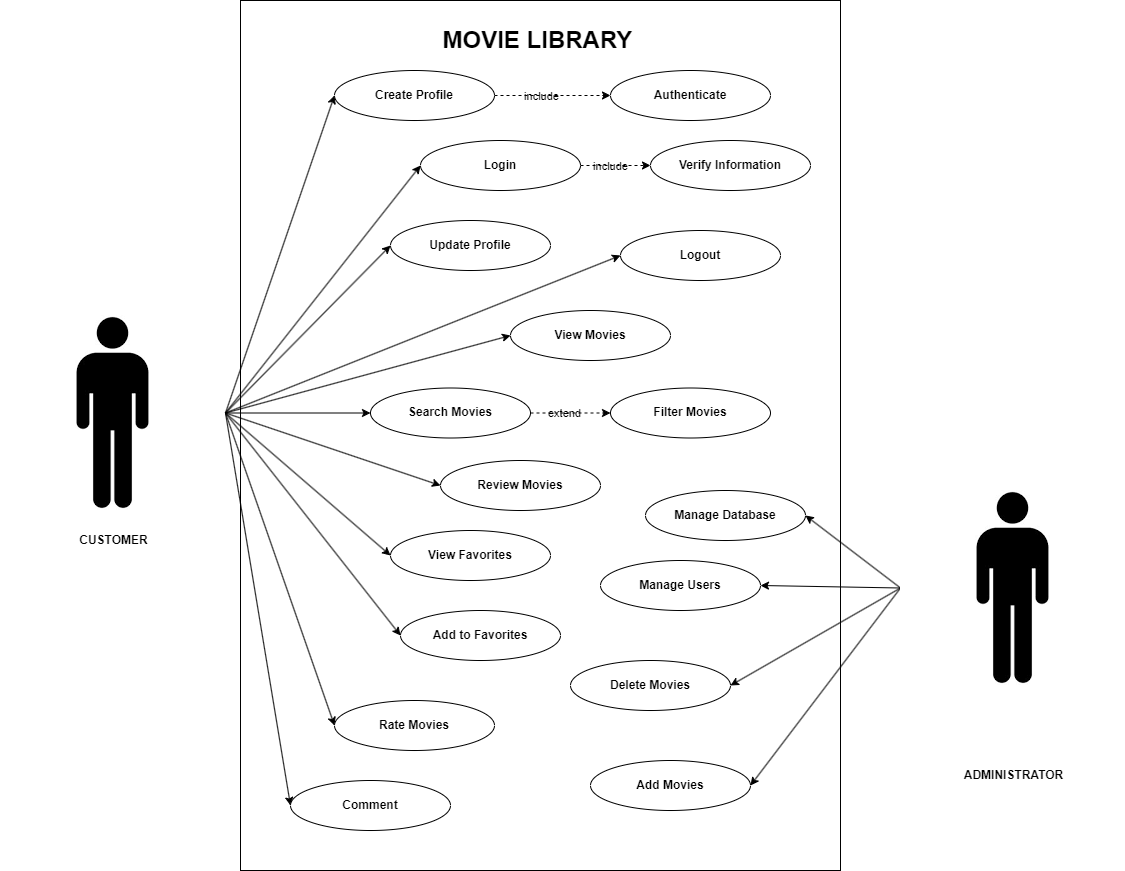
\includegraphics[scale=0.40]{images/USE CASE WET.drawio.png}\\[0.1cm] 

\clearpage
\myparagraph{Appendinx 2} ERD Classes

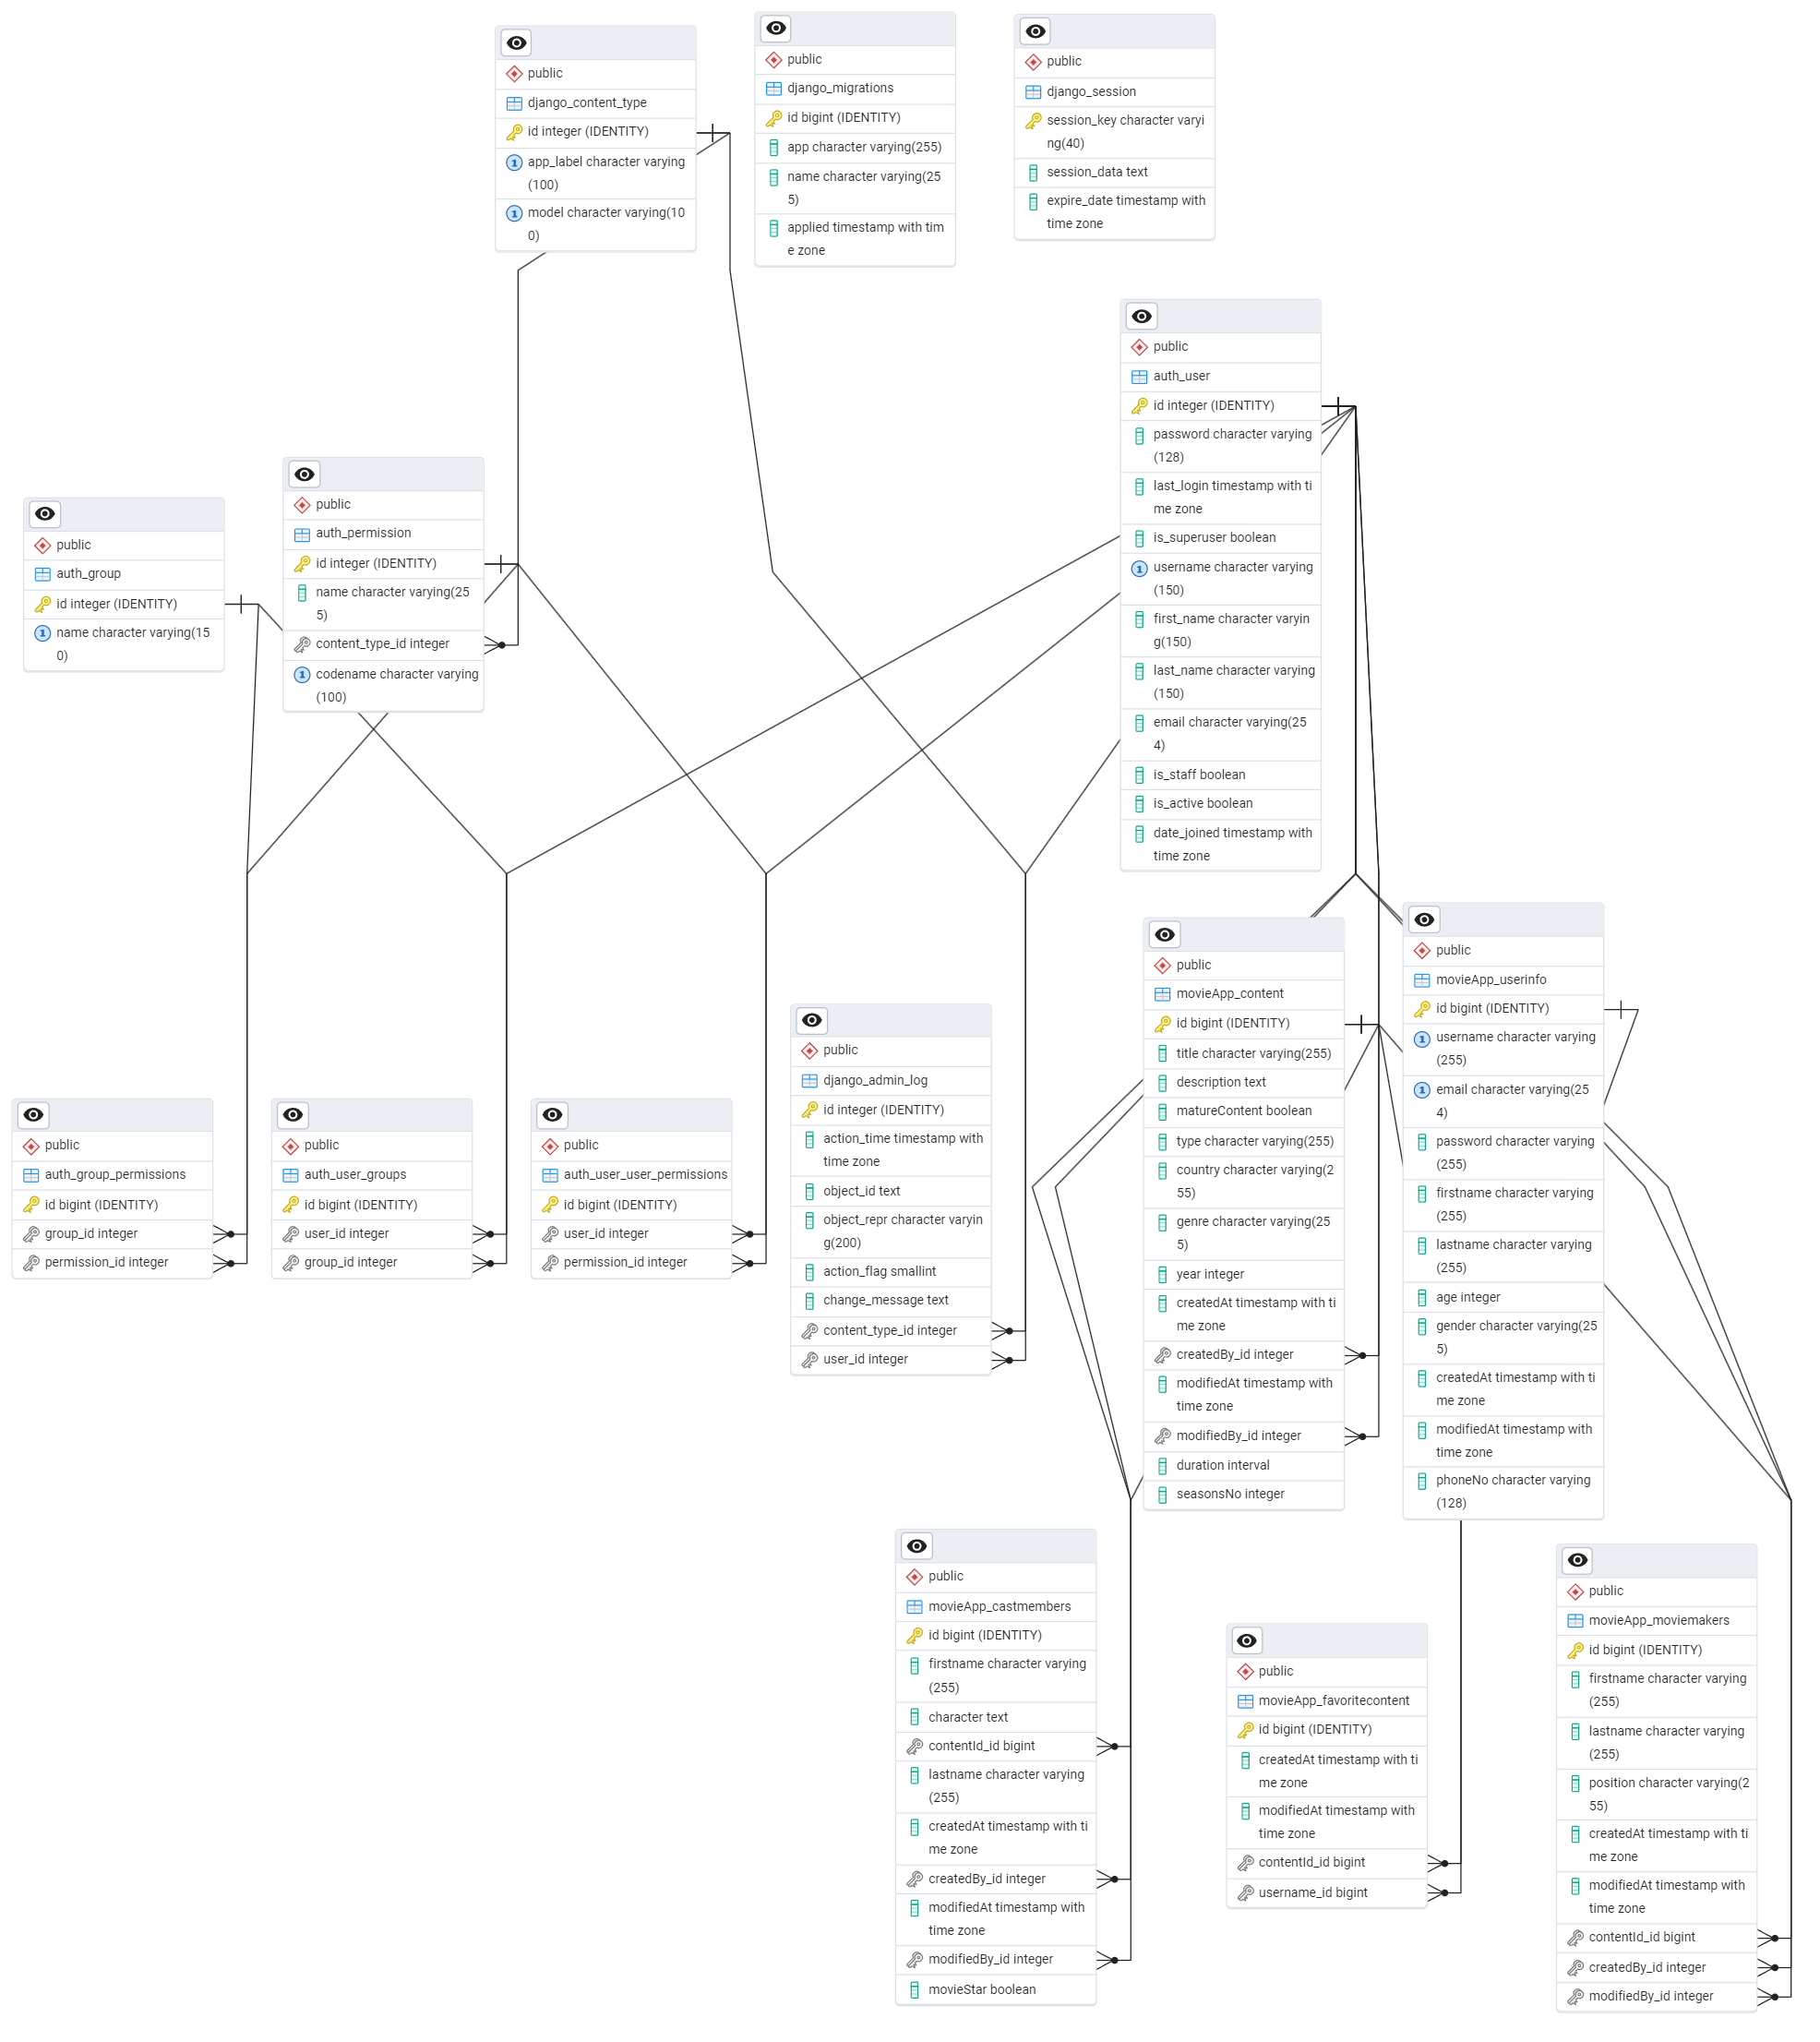
\includegraphics[scale=0.24]{images/ERDNewUpdated.png}\\[0.1cm] 

\clearpage
\myparagraph{Appendix 3} ERD Overview

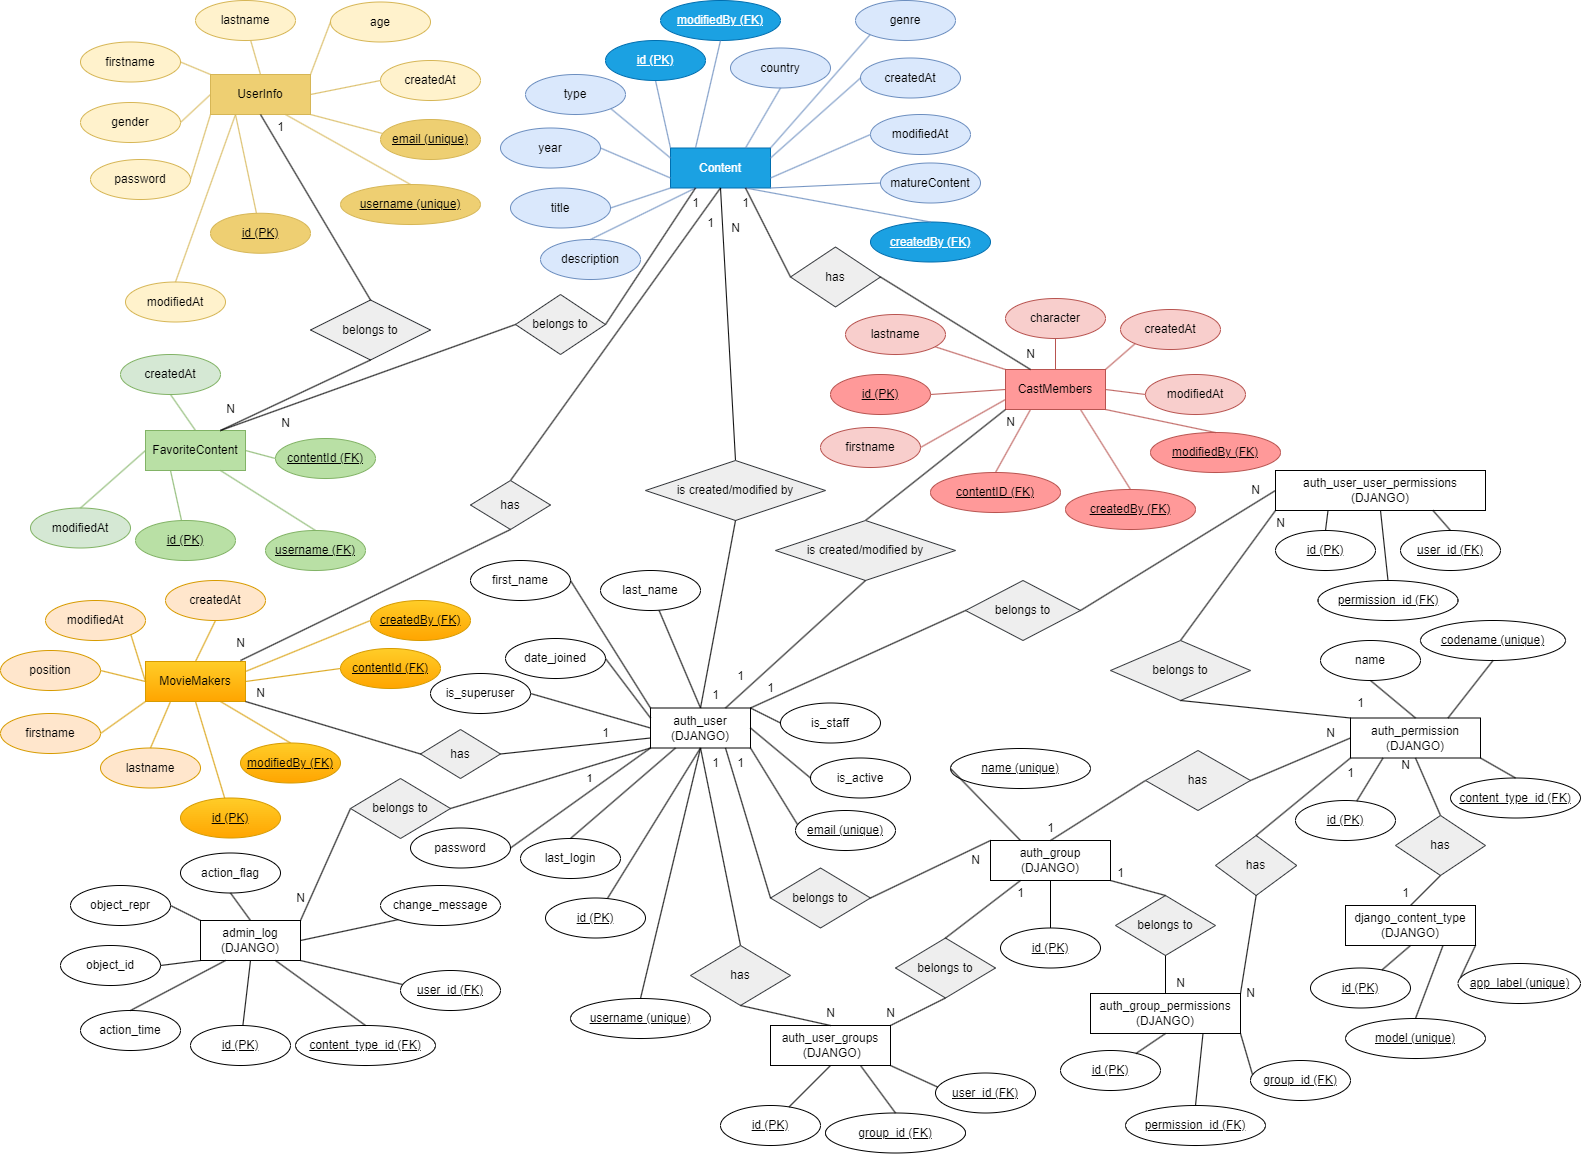
\includegraphics[scale=0.30]{images/WebTechERDNewUpdated.drawio.png}\\[0.1cm] 

\clearpage
\myparagraph{Appendix 4} 

\end{document}

